\documentclass[12pt,a4paper,english,onecolumn]{IEEEtran}

\usepackage{datetime}
\usepackage{caption}
\usepackage{graphics}
\usepackage{graphicx}
\usepackage{minted}
\usepackage{hyperref}
\usepackage[utf8]{inputenc}
\usepackage[paper=a4paper, top=2cm, bottom=3cm, left=2.5cm, right=2.5cm]{geometry}
\usepackage[
    backend=bibtex,
    style=numeric,
    bibencoding=ascii,
    sorting=ynt
]{biblatex}
\addbibresource{bibliography}

\renewcommand*\contentsname{Table of Content}
\renewcommand*\listfigurename{List of Images}
\renewcommand\listingscaption{Example}
\renewcommand{\listtablename}{List of Tables}
\captionsetup[table]{name=Table}
\renewcommand*\figurename{Image}
\usemintedstyle{bw}
\hyphenpenalty=100000
\nocite{*}
\usepackage[T1]{fontenc}

\begin{document}

\title{Cyber Reasoning System}

\author{Claudiu-Florentin GHENEA$^{1}$ and George-Andrei IOSIF$^{2}$\\
$^{1,2}$\emph{Politehnica University of Bucharest, Computer Science Department, Romania}\\
Email: $^{1}$claudiu.ghenea@stud.acs.upb.ro, $^{2}$george\_andrei.iosif@stud.acs.upb.ro}

\maketitle

\begin{abstract}

As the number of devices has increased steadily over the last few decades, so has the number of executables, which are the set of actions that the device's processors must perform. This increase reflected in the attention paid by malicious people (to find security-related issues) and made infeasible the manual vulnerabilities assessments of all the programs.

Automated tools have been developed, and a novel approach has proven its worth in recent years: cyber reasoning systems. These are specialized systems capable of dealing with all aspects of binary program vulnerabilities, including discovery, exploitation, and patching. Following DARPA's Cyber Grand Challenge, in which multiple cyber reasoning systems were opposed against each other to demonstrate their accuracy and efficiency, the majority of them became closed source, unmaintained, or commercial. As a result, the open-source community does not reap the benefits of this novel approach.

We propose a new open source cyber reasoning system in this thesis. Due to the issue's complexity, we are currently targeting only ELF executables built from a C codebase and running on an x86 instruction set architecture.

Given a vulnerable program and no additional information about it, our system will be able to detect flaws using techniques like fuzzing and symbolic execution. The resulting proof of vulnerability will then be used, along with additional information about it, to create exploits with the greatest possible impact. Switching to a defender's perspective, the system will generate a signature for detecting an exploit attempt and a patched binary that can successfully replace the old one, but without the discovered security flaw.

\end{abstract}

\section{Background and Concepts}

An \textbf{executable} is a type of binary file that usually contains machine code (also known as instructions) for a Central Processing Unit (abbreviated CPU) to execute. An executable becomes a \textbf{process} when it is loaded into the memory and the containing instructions are being ran by the CPU.

Nowadays, technology touches \textbf{every aspect of our lives}, from the most basic things as smart fridges, car keys to phones, computers, and servers. Most of the time, everything sums up to a system running some kind of executable. 
Having this in mind, we might want to pay attention to those devices and the security that they provide (implicitly their software) as they could cause major private data leaks such as personal address, bank accounts or pictures.

\subsection{Weaknesses. Vulnerabilities}

\textbf{Weaknesses} are flaws, faults, bugs or other types of errors (for example, buffer-overflow, insecure deserialization, broken access control, etc.) in software or hardware that if left unresolved. They could result in a system being vulnerable to attack.

\textbf{Vulnerabilities} are the entry points for an attacked to gain unauthorized access to a system. Taking control of a system or resource can cause a variety of risks for an individual or an organization. Vulnerabilities can cause disruptions in providing services or even leading to data breaches.

Vulnerabilities often target one or more of the basic concepts of security, namely the CIA triade:
\begin{itemize}
    \item \textbf{Confidentiality}: Assures that all data and resources are protected from any unauthorized type of access. 
    \item \textbf{Integrity}: Assures that type of data is protected from unauthorized changes and it assures that it is correct.
    \item \textbf{Availability}: Assures the uninterrupted acces to a system.
\end{itemize}

These are only a couple of reasons why we should prevent them by using state of the art detection technologies.

\subsection{CWEs. CVEs}

\textbf{Common Weakness Enumeration}\footnote{https://cwe.mitre.org/about/index.html} (abbreviated CWE) is a community-driven list of common types of weaknesses that are found in software or hardware. CWE are organized by categories in a graph-like structure. For example, \textit{CWE-121: Stack-based Buffer Overflow} is identified as follows. It starts from a general weakness category, in this case \textit{CATEGORY: Memory Buffer Errors}, then has a parent node \textit{CWE-787: Out-of-bounds Write} and finally an edge \textit{Stack-based Buffer Overflow} which is the actual CWE.

Each category can be a part of another category, and each node can have multiple parents and links (children). Use of CWE usually helps prevent the security vulnerabilities that could be present in a software or hardware product. For this project, we will use the CWE database to categorize found vulnerabilities.

In the same way as CWE, \textbf{Common Vulnerabilities and Exposures} (abbreviated CVE) is a public database composed of identifiers that uniquely reference a discovered vulnerability. Each identifier contains details such scores, what application and versions does it affect, reference to the weakness and other specific information for that particular vulnerability. 

\subsection{Curent Context}

As software permeates every aspect of our current society, from homes to the infrastructure of critical services in conjunction with the increasing complexity of those systems, security flaws tend to increase as well \cite{hacrs}. \textbf{The number of vulnerabilities has almost tripled in the last years} (2015-2020 graph from NIST)\footnote{https://www.redscan.com/news/nist-nvd-analysis/}. Last year was an especially difficult year, with the rise of ran somewhere attacks and the requirement for a secure remote workforce.

It is described in a Redscan report\footnote{https://www.redscan.com/news/nist-nvd-analysis-2021-record-vulnerabilities/} that in 2021 there were 18.439 vulnerabilities disclosed with an average of \textbf{50 CVEs per day}. It is also mentioned that 90\% of all the CVEs discovered can be exploited by attackers with limited technical skills, and 61\% of all CVEs require no used interaction (for example, clicking a link, downloading or running something) which is raises major concerns about the developing and security assessments that are not being properly done for many of the executables that are being commercialized.

\subsection{Manual Analysis is no Longer Possible}

Initially the analysis of security flaws has been a manual process, experts spend \textbf{significant time analyzing software}. The requirement for tools to automate some of the tasks that are part of a security assessment is growing, related to the amount of software to be analyzed. Even though human analysts are already taking advantage of this kind of automation tools, the aforementioned growth in software that requires to be analyzed has \textbf{reached the scalability limits} of the manual analysis. Thus, the attention has turned to automated program analysis that has as goal identifying and fixing issues present in software at a large scale.

In an effort to drive research and development to this kind of automated analysis programs known in the literature as Cyber Reasoning Systems, DARPA sponsored the \textbf{Cyber Grand Challenge} (abbreviated CGC), a competition to show the current state of the art in this area. Those systems combine various tools and expert knowledge to create an automonus system that performs \textbf{vulnerability detection, exploitation and patching} without the requirement of a human attendance, as a contrary to the initial manual process. Details regarding this challenge finalists and their projects will be covered in the following chapter.

As the solutions that have emerged from the DARPA's CGC were in the form of a tool that a human expert could use to conduct a security assessment, they did not perform as well as a human expert when evaluated in a vulnerability analysis competition (namely the DEFCON CTF) as the autonomous systems could not easily understand the underlying logic of certain applications. Having this as a start point, a team of researchers \cite{hacrs} approached the idea of developing a \textbf{human-assisted CRS} to which an expert or even a non-expert could help the system to fill the semantic gap in the analysis of complex applications. Depsite this makes the tool supervised, there were better results.

\section{State of the Art}

\subsection{For Cyber Reasoning Systems}

In this chapter, we will go on to present the papers from DARPA's CGC finalists, as well as covering some details about the contest. As aforementioned, CGC was a competition with the purpose of \textbf{showcasing the current state of the art in systems that perform automated vulnerability detection}.

This competition was modeled like a game in which each CRS was responsible for a server running the same set of vulnerable software with the purpose of attacking other systems and defending their own, similar to a Capture The Flag (abbreviated CTF) contest. As the challenge also addressed the requirement for a common platform and dataset by which to evaluate CRS, a \textbf{custom operating system}, DECREE, was used to run the services and the set of used binaries is publicly available.

From all the above implementation, only Mechanical Phish and HaCRS are open source, and their codebases can be found on Github. All the DARPA's CGC finalists showcase the potential of cyber reasoning systems and approach mostly similar ways in their both offensive and defensive strategies, the main difference being in the way they implemented the decision-making of the systems to better suit the competition and to win more points. The way they approached the scoring systems and modified the CRS to better suit their approach is also described in the paper, but we only focused on the technical details of the implementation.

\subsubsection{Mayhem}

Mayhem \cite{mayhem} is an automated system for discovering vulnerabilities in a binary. It also verifies them by generating a working exploit or by causing the application to crash. Mayhem was developed by ForAllSecure \cite{mayhem_code} and is the \textbf{winner} of the DARPA's CGC. As a CRS must be capable of both detecting and patching vulnerabilities, the paper describes both modules, and we will cover them one by one. 

The Mayhem's defense mechanism confirms software flaws with the aforementioned approach by verifying if the application crashes or manifests exploitable behavior. Given the fact that Mayhem does not have access to the source code of the application, it will perform \textbf{binary patching} after correctly identifying the vulnerable branch and generating a way to mitigate it. For the mitigation, it is described that Mayhem will add checks only along the code path that it crashes and uses formal methods to only keep the checks that are proven necessary in a try to not affect performance of the binary.

For performing the patching, Mayhem uses two techniques.  The first one is \textbf{full-function rewriting} (abbreviated FFR), in which the whole function is being rewritten and then adjusting all the addresses and offsets withing the program accordingly. The other patching technique is \textbf{injection multipatching}, this being a more conservative approach by substituting a branch instruction at each location that requires patching, by making a jump into a custom location appended to the end of the program that holds instructions from implementing the path.

Mayhem's offense capabilities revolve around generating test cases that trigger some type of unwanted behaviour (any types of flaws) with the help of fuzzing. It is described that a combination of tehniques are used, namely \textbf{greybox fuzzing} and \textbf{white box symbolic execution}.

American Fuzzy Loop (or simply AFL)\footnote{https://github.com/google/AFL} was used for \textbf{fuzzing} with the usage of FFR tehnique to insert the necessary instrumentation (code coverage tracking and reporting mechanisms used by AFL) into the binary and to make some performance improvements. When the FFR failed, they were restrained to use a modified version of QEMU with a huge performance hit (from 100 to 900\%).

As for the \textbf{symbolic execution}, a hybrid version was used that benefits from the strengths of both online and offline symbolic execution. In order for the offline symbolic execution to explore paths, it has to run it twice, the first time symbolically and the second time concretely. On the other hand, offline symbolic execution searches and executes all paths in a single run by forking at each branch. On top of this hybrid approach, Mayhem uses a technique called Veritesting \cite{enhanced_symex} to prevent path explosion by merging similar seeds while preserving the same exploration.

\subsubsection{Xandra}

Xandra was the \textbf{second finalist} of the DARPA's CGC that was developed by a team called TECHx, composed of people from GrammaTach, University of Virginia and Microsoft \cite{xandra}. The format of the publication is similar with the Mayhem one, describing the strategy they have used, the defense mechanism and the offensive one, also they included the architecture of the software that Mayhem did not. Similar as before, we will describe the offense and defense of this particular CRS.

Firstly, we will start with the architecture. Xandra implements components that serve different purposes. The core of the architecture is the GameMaster component which is in charge of managing the work, making interactions with the DARPA interface (submitting patched binaries, proof of vulnerabilities and others) and managing the work of other components.

The offensive component is composed of \textbf{fuzzing} pods and a proof of vulnerability (abbreviated PoV) generator that converts crashes into PoVs. The defensive component, called Helix, is responsible for \textbf{analyzing binaries}, \textbf{adding security policies to the binaries} and \textbf{deploying} Intrusion Detection System (abbreviated IDS) \textbf{rules}, method that was not used by Mayhem. In Layman's terms, Helix component is in charge with altering the binary in any way and to generate IDS rules. The last component is Daffy, the dynamic analysis engine that generates the patches to be applied by Helix.

Xandra's offense revolves around \textbf{fuzzing} and \textbf{symbolic execution}, similar to Mayhem. For this, they used OpenStack cloud management\footnote{https://www.openstack.org} infrastructure and ran multiple pods, each pod containing multiple instances of their custom AFL and one instance of the symbolic execution engine. The necessary seeds for AFL were provided via a capture file from the network, on which they used a proprietary technique called (de)noncification to get better seeds as input for AFL. As AFL requires to monitor the program, profiling was used in the form an emulation and binary instrumentation, the binary instrumentation being the more efficient one. To speed up the process, they have removed from the binaries redundant system calls, sleeps and did some tweaking with the \mintinline{text}{fork()} function of AFL. Given the fact that fuzzing can sometimes be ineffective in finding some hidden paths or getting pass some crafted checks, a symbolic execution engine was designed called Grace to augument AFL. Grace will select inputs generated by AFL and attempt to modify them to drive the program towards new edges. 

Xandra's defense is provided by the two aforementioned components. Helix can efficiently \textbf{rewrite binaries} without accessing their source code. The main transformations used are block-level instruction, point-patching binary optimization and selective Control Flow Integrity (abbreviated CFI). The second component, Daffy, is the dynamic analysis engine that \textbf{generates rules for faulty instructions and bounds for stack arrays}, thus providing patches for Helix to apply. It is mentioned that Daffy was inspired by Howard \cite{howard}. Daffy builds up a database of memory access patterns for non-crashing inputs and compares them with memory accesses that cause the binary to crash. Based on the said difference, Daffy can generate policy rules to be applied so that crash will be mitigated.

\subsubsection{Mechanical Phish}

Mechanical Phish \cite{mechanical_phish} was the \textbf{third finalist} of DARPA's CGC and was developed by a team of researchers from various universities. The publication respects the same pattern as Mayhem and Xandra, starting with their team management, architecture, offense and defense.

Mechanical Phish's architecture was heavily based on isolation by using \textbf{Docker containers}\footnote{https://www.docker.com/} and \textbf{Kubernetes}\footnote{https://kubernetes.io/} as orchestrator to ensure scalability, availability and ease of deployment. For this project, they leveraged a variety of open source components, the most important ones being \mintinline{text}{angr}\footnote{https://github.com/angr/angr} and Driller\footnote{https://github.com/shellphish/driller}. \mintinline{text}{angr} is a binary analysis framework used by Driller to implement concolic execution in conjunction with the well-known AFL. In their architecture, Driller along with other tools compose the Worker module that is in charge of the program analysis\footnote{https://github.com/mechaphish/mecha-docs}.

Other components that are part of the architecture are: Rex for automated exploitation, Meister for scheduling the tasks, Scriba for deciding what exploits and patches to submit to Ambassador. The Ambassador is in charge of communication with the CGC API to retrieve challenge binaries, submit PoV and other details related to the challenge.

Mechanical Phish's offensive involves two steps. The first step is crashing the binary with the usage of \textbf{fuzzing} combined with \textbf{symbolic execution} (the Driller component) and the second step is finding a way to modify the input generated at the first step to produce exploits. It is described that they came up with a list of crash types and methods to exploit those, from this list pointer overwrite, arbitrary read/write and \mintinline{text}{vtable} overwrite are mentioned. They also provided an example of a simple buffer overflow and explained how symbolic execution and fuzzing can detect it, after generating the crash at the first step. In the second step, the given crash will be symbolically traced and the system will then try to make a jump to a zone in which code can be injected. This is achieved with the help of a \textbf{constraint solver}.

For the patching part, they implemented a component named Patcherex built on top of \mintinline{text}{angr}. It adds patches to the binary in an reassembled form \cite{ramblr} and then regenerate the binary. For this paths, in an assembled form, they have implemented three types of techniques to preserve the original functionality and performance of the binary:
\begin{itemize}
    \item \textbf{Binary herdening}: In this technique, they have implemented encryption for the return pointer and additional checks of the transmitted data for preventing memory-leaking exploits.
    \item \textbf{Anti-analysis}: This technique is more related to the competition as it prevents rivals from analyzing their patched binaries by triggering bugs from the emulation environment (via QEMU) along with introduction of backdoors in case some other team would use their binary.
    \item \textbf{Binary optimization}: To increase the performance of the binary and leave more room for the overhead that patching of real bugs might add, they applied optimization such as constant propagation or dead assignment elimination. They noticed that originally the binaries were compiled without compiler optimizations.
\end{itemize}

\subsubsection{HaCRS}

A team of researchers approached the idea of developing a \textbf{human-assisted CRS} in the paper \cite{hacrs} by making the software supervised and thus not independent, with the potential of having better results. Their idea came from observing the finalists of the DARPA's CGC performing in a vulnerability analysis competition held by DEFCON that also included human teams. In this competition, the autonomous systems underperformed by not easily understanding certain application, thus struggling to produce valid inputs that would drive the program to a vulnerable state. When humans were able to provide some guidance for the input, the results that followed "\textit{were surprisingly good}" \cite{hacrs}.

For their implementation, they extended Mechanical Phish and tested it in the same environment, namely a part of the binaries on DECREE OS. In the implementation, they leveraged the human part for tasks that are difficult to automate as it relies on human input to provide new ideas when the system gets "\textit{stuck}".

Human interaction was added into the \textbf{discovery stage} of the Mechanical Phish workflow, and it is done via a graphical interface that differs on the level of expertise the human possess. As humans interact with a targeted binary to generate \textbf{input}, those inputs are \textbf{syncronized} throughout the components and can be used to later provide \textbf{suggestions} for other \textbf{users}, those suggestions are also accompanied by the random suggestion that the system provides. They have categorized those types of inputs and outputs as follows:
\begin{itemize}
    \item \textbf{Human-to-automation}: The produced inputs are syncronized with the automated components and used to mutate new inputs.
    \item \textbf{Human-to-human}: Humans can view and modify other test cases provided by others in a collective effort to understand the program and achieve a better code coverage.
    \item \textbf{Automation-to-human}: The resulting mutated inputs can be shown to humans to possibly provide a better understanding of the program. The mutated inputs generated are shaped into a readable form. In the graphical interface they provided a brief program description, some instructions about the task, examples of past interactions and the CRS-generated suggestion.
\end{itemize}

For testing, they have selected only binaries with high semantic complexity to showcase the impact of the input provided by non-experts and semi-experts. The experiment was run in different configurations, the one that we are going to present is the \textbf{symbolic-assisted fuzzing}, this is the reference configuration of the Mechanical Phish, and the \textbf{human-assisted Symbolic-assisted fuzzing} configuration, in which the human assisted component is added. \textbf{Human-assisted symbolic-assisted fuzzing} benefits from both the input of semi-experts and non-experts and because of the \textbf{Human-to-human} approach, the input from semi-experts helped non-experts to have a better understanding of the analyzed binary.

The results were in the favor of the latter, finding twenty more bugs and having 53.45\% more code coverage for the binaries with a higher semantic complexity. This study proved that for binaries with more complex input, CRS could benefit from the insight of non-expert humans. They mentioned that the "\textit{systems are able to operate fully autonomously, just with a lower effectiveness}" \cite{hacrs}.

\subsection{For the Used Technologies}

\subsubsection{Attack Surface Approximation}

We find out that the field of approximating the attack surface of an executable is not a mature one. The only studies related to this topic are written by Christopher Theisen (for example, \cite{automated_approximation}) and discover the attack surface by analyzing the call traces extracted from memory dumps of crashes.

\subsubsection{Fuzzing}

Fuzzing is one of the most popular solution for discovering vulnerabilities, as it is \textbf{providing randomly generated input} to a program while monitoring it for crashes to be triggered. In other words, it is a method to discover software security vulnerabilities by automatically generating input that might be syntactically or semantically incorrect, then feeding it to the effective software \cite{fuzzing_survey}. Fuzzing is responsible for the vast majority of remote code execution and privilege escalation bugs found in security-critical software, thus becoming a mainstream practice in software security\footnote{https://github.com/aflnet/aflnet}.

\subsubsection{Dynamic Taint Analysis}

As it was presented in detail in \cite{dta_essay_repo}, dynamic taint analysis is the silver bullet for tracking the data as it flows inside a process internals. We consider that the dynamic taint analysis, as applied to binary programs, reached a stable state as it achieved good accuracy and now the academia works on increasing it near the ceiling of 100\% and using it on different programming languages and platforms.

Regarding integration in tools from which the industry could benefit, TaintCheck was firstly proposed in 2005. More recently, tools such as Airbus's bincat\footnote{https://github.com/airbus-seclab/bincat} and rtaint\footnote{https://github.com/Cycura/rtaint} were published on the open source community.

\section{Issues. Opportunities}

\subsection{Issues}

During our research, we noticed that although the aforementioned project were successful in DARPA's contest, they are \textbf{not maintained anymore}. The last commits date back from 2019 and those projects are also archived. We were unsuccessful in finding an open source alternative that is still maintained and up to date with the \textbf{latest tools that have emerged} since 2016.

There is a sole exception: Mayhem. It is in a continuous development as it migrates to the commercial environment \cite{mayhem_code}.

Another issue might be the fact that these projects are \textbf{targeting DECREE OS}. None of them are adapted to work on common operating systems, like Linux.

\subsection{Opportunities}

We consider that this is a \textbf{great research opportunity} as this type of automated vulnerability detection, exploitation and patching systems are essential in the context of today's society as mentioned in the first chapters. As a bold statement, it is not only required, but mandatory to reposition the research attention to this area in the context of the latest state of the art open source tools that are available and that can be taken advantage of.

In addition, the \textbf{industry could benefit} from a Linux-based cyber reasoning system as it is the most common operating system used in both development and production.

\section{Project Overview}

We have shown above that cyber reasoning systems are holistic approaches to manage all the aspects related to vulnerabilities in executable files. As the solutions considered, at the moment, state of the art are either unmaintained or closed source (even commercial, as the case of Mayhem, the winner of DARPA's CGC), we propose with our thesis a \textbf{novel open-source CRS} that uses the latest advances in the fields of binary analysis, from both the academia and industry.

The \textbf{variety in the binary analysis} is high, due to various aspects:
\begin{itemize}
    \item Processor's architecture: Bit count, instruction set architecture (abbreviated ISA);
    \item Operating system: System calls;
    \item Binary file format: The effective way of representing the opcodes; and
    \item Programming language: Vulnerabilities classes. 
\end{itemize}

Because we want to implement a \textbf{proof of concept} for a CRS that integrates all the latest improvement, we do not target all the variation in the aspects above. Instead, we want at first to achieve the holistic vulnerability assessment only for \textbf{ELF} files (namely a \textbf{Linux} operating system), build from a \textbf{C} codebase and run on a \textbf{x86} ISA.

\subsection{Core Objectives}

The goals of this system is to \textbf{find}, \textbf{patch}, \textbf{exploit} and \textbf{protect binaries}. Seeing the CRS as a blackbox, without detailing in greater details its functioning (a thing that we will do in the following section), its input are vulnerable programs. Relying on different binary analysis techniques, the CRS then detects its vulnerability, producing \textbf{proofs of vulnerabilities} (abbreviated PoV), each of which triggering a certain vulnerability.

However, the vulnerabilities are limited by constraints accidentally imposed by the executable, namely its shape (for example, the allocated segments and their permissions) and functioning (for instance, some transformations that are applied to the user's input). These constraints are modeled to \textbf{detect which is the greatest impact} that an exploit can have. With this model of the space in which the exploit resides, our CRS will generate a \textbf{payload} which will have a high impact considering the constraints that are present.

For a defender point of view, even if it knows about a given vulnerability (via the PoV), he could not act accordingly. Here, the CRS will help by generating a new version of the program, with the vulnerable parts patched. This can be achieved by analyzing the PoV, determining the root cause of the vulnerability, and rewriting that weak functionality.

In addition, the proof of vulnerability can be further analyzed to detect what are its fundamental characteristics, without which an exploit could not function properly. This information helps to protect a binary program that could not be easily replaced with a patched executable, by creating \textbf{signatures}. These can be concrete, if we talk about a byte sequence in a packet, that can be detected (and blocked) by a network intrusion detection and prevention systems (abbreviated IDPS), or behavioral, as in the case of the host IDPS, which looks, for example, at the parameters of the system calls made by active processes.

\subsection{General Architecture}

Each function we describe in the previous section has a direct correspondent in the overall architecture. It can be seen in the above diagram what are the major modules and how the cyber reasoning system is interacting with the environment it functions.

\vspace{0.3cm}
\begin{center}
    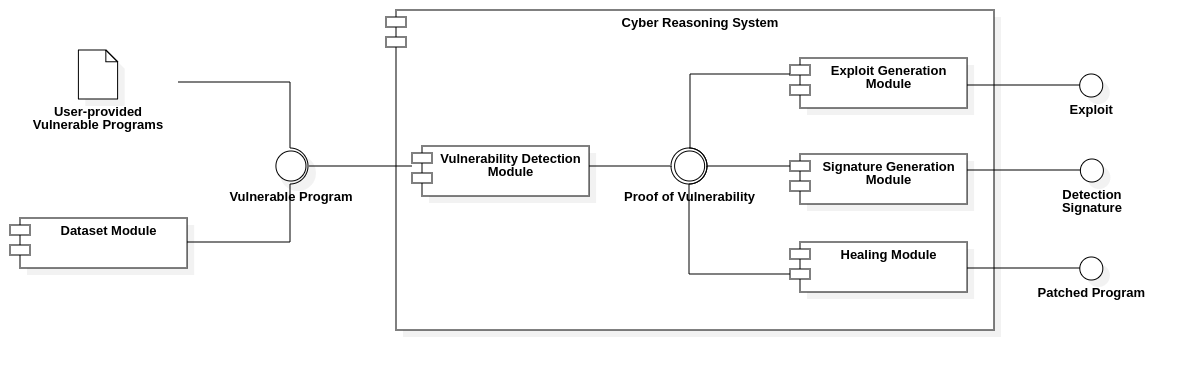
\includegraphics[width=14cm]{images/architecture.png}
    \label{fig:1}
    \captionsetup{justification=centering,margin=1cm}
    \captionof{figure}{The proposed architecture}
\end{center}
\vspace{0.3cm}

To further describe them, each module is seen as a system in which some \textbf{inputs} are processed by some inner processes (which are consistent with the \textbf{purpose} of the module) and later combined into a set of \textbf{output} data. In addition, we will detail which \textbf{techniques} we want to use as a base of our CRS and which ones will be placed in a backlog, consulted when wanting to add extra functionalities or encountering difficulties with the already-chosen ones.

\subsubsection{Dataset Module}

The dataset module \textbf{contains vulnerable programs} generated by us or taken from well-know public test suites. For example, NIST Juliet is integrated, which contains a set of small test programs written in C and exhibiting numerous classes of errors \cite{juliet_testcase}.

Besides the advantage of having the original source code files, these test cases offer indexes where the programs are tagged with their compilation flags and corresponding \textbf{CWEs}. This allows the module to create executables and to \textbf{filter} the whole dataset by specific vulnerabilities, that can be further analyzed by the CRS.

\subsubsection{Vulnerability Detection Module}

The next module in the pipeline is the vulnerability detection one. It takes as input a vulnerable binary program and \textbf{generates proofs of vulnerability}, namely inputs that can be passed to the program to make it behave insecurely. In addition, information could be offered to describe in more detail the \textbf{root cause} of the vulnerability.

There are multiple steps and approaches that can be integrated in this module:
\begin{enumerate}
    \item For \textbf{determining the attack surface} (the search space)
    - \textbf{Static analysis} of the executable: It can be said that if a program uses an input stream, then the executable will contain some evidence. For example, if we consider reading from files, then functions such as \mintinline{text}{read}, \mintinline{text}{fread} and \mintinline{text}{fscanf} are linked (statically or dynamically).
    - \textbf{Behavior analysis of a process}: By observing the way in which a process behave, it can be determined what are the inputs that the program takes. For instance, if the \mintinline{text}{recv} syscall is called, it can be certainly said that an attack vector is networking.
    - \textbf{Crash reporting} (as in \cite{automated_approximation})
    \item  For \textbf{limiting the search space}
    - \textbf{Binary diffing}: Between releases, software vendors adds new functionality to their programs, in order to better solve the end user issues. So two consecutive versions of the same program can be different. Besides these changes, another ones can appear due to the fact that the vendors continuously find out about vulnerabilities in their software and patch them. By comparing two versions of the same program, vulnerabilities can be discovered either in the new functionalities (the older codebase is ignored and considered, in this scenario, invulnerable) or in the oldest version, by determining the security patches of the newest version.
    - \textbf{Behavior analysis of a process}: The same behavior analysis described above can determine the hotspots of the program, namely the instruction that are frequently used by the process. These can be analyzed with priority because there is the highest triggering probability.
    \item  For searching the space to \textbf{find out vulnerabilities}
    - \textbf{Fuzzing}: By giving specific inputs (random or generated via some heuristics) to the program, via the input streams determined in the attack surface approximation step, the program could behave insecurely (crashing, producing segmentation faults).
    - \textbf{Symbolic execution}: The concrete values that are passed to the program in a normal execution could be replaced with symbolic ones to determine edge cases. 
    - \textbf{Crash reporting}: The technique of reporting crashes to development teams (in order to fix the behavior that produced them) can be used here too. These can be produced by user activity, program's bugs, fuzzing or exploited vulnerabilities. A crash can be, for example, the result of an overwrite of a function pointer (which is a security issue too, not just a functional one) that is later called.
    \item  For \textbf{finding the root cause} of a vulnerability
    - \textbf{Dynamic taint analysis} (abbreviated DTA): By running again the program with the PoV that was found in the last step, but under extra observation (for example, by tracing all the operations), dynamic taint analysis determines how the tainted information (the one from the input) reached the sensitive position of memory that triggered the vulnerability.
\end{enumerate}

\subsection{Exploit Generation Module}

As we described in the "\textit{Core Objectives}" section, having a vulnerability does not mean that an attacker could achieve anything he wants. It is limited by other factors, imposed unintentionally by the shape and the behavior of the executable. This module deals with \textbf{modeling these constraints} by taking as input the binary, a PoV and some additional details about it (for example, the DTA-determined root cause).

It then uses some \textbf{strategies} (based on \textbf{game theory} and \textbf{boolean satisfiability problem}) to \textbf{generate an exploit} that will have the highest impact on the exploited system. For example, a \mintinline{text}{read} syscall that produces a buffer overflow, but which has a small \mintinline{text}{count} argument, will require an attacker to build a compact, but impactful return oriented programming chain, based on the gadgets that the executable contains.

\subsection{Signature Generation Module}

Same as the Exploit Generation Module, the Signature Generation one uses the same input information, but with a different goal: to \textbf{generate efficient signatures} to protect a system running a vulnerable program against exploitation attempts. This is due to critical or obsoleted systems, which does not support a software update due to the interruption of the services or old operating systems or hardware, which not enable newer and safer functionalities (for example, \mintinline{text}{gets_s} usage, which was introduced in the C11 standard).

The module relies on the additional information about the PoV, generated, for example, by dynamic taint analysis. In this way, only the fundamental byte sequences of the proof will be included into the signature, a strategy that will ensure a greater false positive rate.

\subsection{Healing Module}

The last module that produces an output useful to the end user of the CRS is the healing one. The same information as the above two modules is used to determine what aspect of the binary is vulnerable. This can vary from a section that is marked as executable (and that, due to a buffer overflow, could allow an attacker to execute shellcodes) to an incorrectly-used format string function.

Via \textbf{binary rewriting} techniques and custom \textbf{patching heuristics}, the module will be able to \textbf{create a new executable} which is no longer vulnerable and that could be deployed instead of the actual, vulnerable one.

\section{Current Status}

In this semester, our efforts were divided in \textbf{two directions}, research and implementation, which we will detail below.

As the concept of cyber reasoning system was new for us, we invested time in understanding its purpose and architecture. This was done by \textbf{researching the field of CRS}, ultimately finding about DARPA's Cyber Grand Challenge. We studied the \textit{modus operandi} of the competitions itself and its participants, paying greater attention to its winner by reading research and blog posts and, in some cases (for instance, Mechanical Phish and HaCRS), discovering the repositories with source code.

After that, we \textbf{propose the architecture} that the "\textit{General Architecture}" section presented by integrating the technologies that we found to be relevant in the current days: fuzzing, symbolic execution, dynamic taint analysis and more. As it is a premature modelling of a complex problem, we are expecting that the next iterations of this document to present a different, but more mature architecture of our CRS.

We then made the pragmatic decision to \textbf{split our work in iterations}, each iteration having as a deliverable a module of the CRS. So, for each of them, we want to first study the state of the art of the domains that the component involved, discover available open source tools, and then start the effective implementation. For example, the exploit generation module implies a prior research on that field, some accommodation with tools such \mintinline{text}{angr} and \mintinline{text}{pwntools} and only after the work on our CRS.

At the moment, we managed to create a GitHub organization \cite{crs_org} that is hosting the repositories for all the module we already finished:
\begin{enumerate}
    \item \textbf{Dataset Module} \cite{dataset_repo}: We created hundreds of vulnerable executables from two open source test suites, namely NIST's C Test Suite \cite{nist_c_test_suite} and Juliet \cite{juliet_testcase}. These we're wrapped into a standardized folder structured and managed by a Python 3 script that deals with the compilation and their filtering based on CWEs.
    \item  A submodule of the \textbf{Vulnerability Detection Module}, \textbf{Attack Surface Approximation} \cite{surface_repo}: This submodule deals with the static analysis of the input binaries for discovering their attack surface, namely the input mechanism they use. It is helpful for activating the next modules in the pipeline of the CRS. We achieve this by using the API of a popular reverse engineering tool, namely NSA's Ghidra, and verifying some necessary condition for an executable to use a specific input stream. For instance, if the executable does not interact with the program's parameters (the \mintinline{text}{main()}'s arguments, \mintinline{text}{argc} and \mintinline{text}{argv}), then a fuzzer modifying some (inexistent) parameters is useless.
\end{enumerate}

It is worth mentioning to be mentioned that the latter is required due to our goals. In comparison to the cyber reasoning systems proposed at Cyber Grand Challenge, which deal with an executable taking input only from network packets, our CRS is meant to discover vulnerabilities in all major input streams, \mintinline{text}{stdin} and arguments included.

Besides this, we profited from homeworks that we had for our university classes and studied multiple topics that will be included in the CRS we are developing. This effort resulted in three essays, two of them being referenced above:
\begin{itemize}
    \item Generic fuzzing;
    \item Network fuzzing \cite{network_fuzzing_essay_repo}; and
    \item Dynamic taint analysis \cite{dta_essay_repo}.
\end{itemize}

\section{Further Planning}

We want to dig deeper into the \textbf{state of the art} of several techniques, including fuzzing, symbolic execution, and dynamic taint analysis. These topics will be documented in the next iteration of this document and will be included in the module that we believe is the most difficult: vulnerability detection.

Despite the challenges, we want to \textbf{complete that module} by the end of the next semester. Taking this into consideration, our CRS will be able to extract vulnerable programs from a dataset, discover their attack surface and vulnerabilities, and provide a detailed analysis of the root cause of the security issue.

\section{Bibliography}
\nocite{*}
\printbibliography[heading=none]

\end{document}